% !TeX program = xelatex
% Compile main.tex with XeLaTeX twice or with Tectonic.
\documentclass[11pt,a4paper]{article}
\usepackage[left=2.25cm,right=2.25cm,top=2.25cm,bottom=2.25cm]{geometry}
\usepackage[T1]{fontenc}
\usepackage{lmodern,graphicx,booktabs,tabularx,longtable,array}
\usepackage{float,subcaption,amsmath,amssymb,etoolbox}
\usepackage[table]{xcolor}
\usepackage{enumitem,fancyhdr,titlesec,tikz,listings,microtype}
\usetikzlibrary{arrows.meta,positioning,calc}
\usepackage{hyperref,bookmark,needspace}
\definecolor{Navy}{HTML}{16324F}
\definecolor{Blue}{HTML}{1D6FA5}
\definecolor{Teal}{HTML}{15847B}
\definecolor{Muted}{HTML}{667784}
\definecolor{PaleBlue}{HTML}{EDF6FA}
\definecolor{PaleGray}{HTML}{F5F7F8}
\hypersetup{colorlinks=true,linkcolor=Navy,citecolor=Teal,urlcolor=Blue,
 pdfauthor={Group 15},pdftitle={Group 15 - Experiment 3 Desktop Object Classification and Sorting},
 pdfsubject={HSV simulation workflow, YOLO11 physical sorting, and ROS 2 task control}}
\pagestyle{fancy}\fancyhf{}
\fancyhead[L]{\small\sffamily\color{Muted}Experiment 3: Desktop Object Sorting}
\fancyhead[R]{\small\sffamily\color{Muted}Group 15}
\fancyfoot[C]{\small\sffamily\color{Muted}\thepage}
\renewcommand{\headrulewidth}{0.35pt}\setlength{\headheight}{15pt}
\titleformat{\section}{\Large\bfseries\sffamily\color{Navy}}{\thesection}{0.7em}{}
\titleformat{\subsection}{\large\bfseries\sffamily\color{Blue}}{\thesubsection}{0.6em}{}
\titleformat{\subsubsection}{\normalsize\bfseries\sffamily}{\thesubsubsection}{0.5em}{}
\titlespacing*{\section}{0pt}{1.4em}{0.65em}
\titlespacing*{\subsection}{0pt}{1.1em}{0.4em}
\setlength{\parindent}{1.4em}\setlength{\parskip}{0.22em}
\setlength{\emergencystretch}{3em}
\clubpenalty=10000
\widowpenalty=10000
\displaywidowpenalty=10000
\setlist{leftmargin=2em,itemsep=0.16em,topsep=0.3em}
\renewcommand{\arraystretch}{1.2}
\captionsetup{font=small,labelfont=bf}
\raggedbottom
\newcolumntype{Y}{>{\raggedright\arraybackslash}X}
\newcolumntype{L}[1]{>{\raggedright\arraybackslash}p{#1}}
\newcolumntype{C}[1]{>{\centering\arraybackslash}p{#1}}
\newcommand{\file}[1]{\path{#1}}
\newcommand{\src}[1]{~\cite{#1}}
\newcommand{\lead}[1]{\par\smallskip\noindent\textbf{#1}\ }
\newcommand{\tabstart}{\centering\small\setlength{\tabcolsep}{5pt}}
\lstset{basicstyle=\ttfamily\footnotesize,breaklines=true,columns=fullflexible,
 backgroundcolor=\color{PaleGray},frame=single,rulecolor=\color{Muted!35},
 showstringspaces=false,xleftmargin=0.5em,xrightmargin=0.5em}
\begin{document}
\hypersetup{pageanchor=false}
\begin{titlepage}\thispagestyle{empty}
\begin{tikzpicture}[remember picture,overlay]
\fill[Navy] (current page.north west) rectangle ([yshift=-10.6cm]current page.north east);
\fill[PaleBlue!65!white] ([yshift=-10.6cm]current page.north west) rectangle (current page.south east);
\fill[Teal] ([xshift=1.45cm,yshift=-10.25cm]current page.north west) rectangle ([xshift=7.45cm,yshift=-10.45cm]current page.north west);
\end{tikzpicture}
\vspace*{0.65cm}
{\color{white}\sffamily\Large Group 15 Experiment Report\par}
\vspace{0.55cm}
{\color{white}\sffamily\fontsize{29}{35}\selectfont\bfseries
Experiment 3\par Desktop Object\par Classification and Sorting\par}
\vspace{0.5cm}
{\color{white}\sffamily\large Simulation Workflow and Physical Sorting Verification\par}
\vspace{2.3cm}
\renewcommand{\arraystretch}{1.5}
\noindent\begin{tabularx}{\textwidth}{@{}L{3.9cm}Y@{}}
\textbf{\sffamily Course} & Robot Integration Group Project I\\
\textbf{\sffamily University} & Ocean University of China\\
\textbf{\sffamily Class / group} & Group 15\\
\textbf{\sffamily Report type} & Group experiment report\\
\textbf{\sffamily Platform} & Jetson, ROS 2, and mechArm 270\\
\textbf{\sffamily Task} & Six source grids and two sorting areas
\end{tabularx}
\renewcommand{\arraystretch}{1.2}
\vfill{\sffamily\color{Navy}\large\bfseries Revised September 22, 2026\par}
\end{titlepage}
\hypersetup{pageanchor=true}\pagenumbering{Roman}
\section*{Abstract}\addcontentsline{toc}{section}{Abstract}
We built a desktop sorting system for the mechArm 270 using six pickup grids and two placement areas. An overhead camera identifies the object in each grid, and a ROS 2 state machine selects and executes the corresponding taught motion.

The Gazebo and MoveIt simulation uses HSV detection to sort four cubes and two hollow bridge-shaped objects. All six objects reached their target positions, including both bridges. The run took 391.53 s; the monitor recorded 37,831 joint samples with no joint-limit violations or unsafe contact pairs. Grasping uses a fixed attachment constraint after alignment and gripper-closure checks.

The physical system runs YOLO11 on a Jetson. Four cube classes go to the right placement area, while red cuboids and orange bridges go to the left. We use seven-frame histories with five matching group observations to stabilize grid decisions, and 17 taught poses for pickup and placement. The physical demonstration completed six transfers from five initial objects and one yellow-cube re-feed, with all six destination choices correct. Separate empty-cell and unknown-object tests checked the controller's no-motion branch.

The v4 detector's recorded mAP50--95 is 0.8755. A red/pink classifier assists the original detector, and a later red/orange classifier addresses confusion between the cuboid and bridge. The latter achieved 84/84 correct test crops and 36/36 detections in the saved video regression. These image tests are reported separately from robot transfer results.

\vspace{0.6em}\noindent\textbf{Keywords:} object sorting; YOLO11; ROS 2; mechArm; fixed-grid picking; Gazebo

\clearpage\setcounter{tocdepth}{2}
\begingroup
\fontsize{10}{10.4}\selectfont\setlength{\parskip}{0pt}
\makeatletter
\patchcmd{\l@section}{\addvspace{1.0em \@plus\p@}}{\addvspace{0.20em \@plus\p@}}{}{}
\makeatother
\tableofcontents
\endgroup
\clearpage\pagenumbering{arabic}
\section{Experiment Objectives and Requirements}
\subsection{Purpose and connection with Experiment 2}
The aim of Experiment 3 is to make the robot choose a useful action from camera information. In Experiment 2, the main work was recording robot states and replaying a fixed route. The operator already knew the picking and placing points. In this experiment, an object may appear in any of six prepared grids, and its group decides its destination. The system must connect visual detection, task decisions, and robot movement into one repeated process.\src{requirements,lab2}

The task is to identify at least two object groups, select their source grids and place them in the corresponding areas. We use fixed pickup positions, so the camera only needs to identify a cell. The camera, robot base and objects must remain close to the calibrated arrangement.

\subsection{Basic task and required interfaces}
The handout requires four to six fixed source grids and at least two sorting areas. Our implementation uses six grids and two destinations. After the task starts, the operator must not manually choose the object class, source grid, or placement area.\src{requirements}

\begin{table}[H]\tabstart
\caption{Required interfaces and their roles}
\begin{tabularx}{\textwidth}{@{}L{3.0cm}L{5.0cm}Y@{}}
\toprule Interface & Required form & Purpose\\\midrule
Camera image & \file{sensor_msgs/Image} & Provide the scene used for detection.\\
Object detection & \file{vision_msgs/Detection2DArray} & Provide class, box, and confidence.\\
Grasping task & ROS 2 Action or an equivalent long task interface with feedback & Send a request and report progress or failure.\\
Task decisions & State machine or BehaviorTree & Select targets and manage normal and abnormal states.\\
System startup & One Launch file & Start the camera, perception, robot, and task control chain.\\
\bottomrule
\end{tabularx}
\end{table}

The task loop is to observe the table, find a valid object, decide its group and destination, execute picking and placing, and then observe again. Empty grids and unknown classes should be skipped. A failed grasp or unreachable target should lead to a stop or a safe return. Logs should preserve the recognition result, motion result, placement result, and error information.

\subsection{Simulation and physical requirements}
The required order is simulation first, followed by physical verification. Simulation should contain the arm, gripper, overhead camera, table grid, and at least two object groups. The simulated image must pass through the detection and task-control chain. The physical stage uses a fixed RGB camera, a Jetson computer, and the real mechArm. The physical layout must provide six target objects from at least two groups.\src{requirements}

\begin{table}[H]\tabstart
\caption{Acceptance targets stated in the Experiment 3 handout}
\begin{tabularx}{\textwidth}{@{}L{3.1cm}Y Y@{}}
\toprule Item & Simulation & Physical experiment\\\midrule
Sorting performance & At least 5 correctly sorted objects from at least 6 tested objects & At least 5 correctly sorted objects out of 6\\
Class coverage & At least 2 sorting groups & At least 2 sorting groups\\
Autonomy & No manual class, grid, or destination choice after startup & No manual class decision or action triggering during normal operation\\
Abnormal cases & Correctly handle at least 2 types & At least empty grids and unknown objects\\
Motion safety & No clear collision or joint-limit violation & No collision, limit violation, or dangerous action; safe stop on errors\\
Records and startup & Recognition, grasp, and state logs; one Launch & Per-object outcomes and errors; one Launch\\
\bottomrule
\end{tabularx}
\end{table}

The required submission includes the ROS 2 project, Launch and dependency files, trained weights, class definitions, grid configuration, task-control description, simulation and physical videos, test records, and this report. The task records link each selected target to its motion request and outcome.

\subsection{Experimental setup}
Our physical system uses six source cells and two destinations. The instructor accepted a test starting with five objects and re-feeding the yellow cube once, giving six transfers in total. The final simulation contains four cubes and two bridges. Its normal run and the earlier exception tests are described in Section~\ref{sec:simulation}.\src{simbridge,simbridgerun,simruns}


\section{System Design and Working Environment}
The hardware, labels, and interfaces in this section describe the physical system. The separate final simulation uses HSV detection, four red/blue cubes, two orange bridges, and MoveIt execution as detailed in Section~\ref{sec:simulation}; its topics and class mapping should not be substituted for the physical configuration.

\subsection{Hardware and communication}
The system has three main parts. The Windows computer starts the experiment and shows the camera preview. The Jetson runs the detector, the ROS 2 task controller, and the robot worker. The mechArm performs the joint movements and gripper actions. Keeping the decision and control programs on the Jetson avoids sending every small movement through the Windows preview connection.\src{defense,integration}

The supplied launcher connects to the Jetson at \file{192.168.55.1}. The worker reaches the arm through the TCP endpoint \file{192.168.100.2:9000}. These addresses describe the laboratory arrangement, rather than a general requirement of the algorithm. The camera image size used for region calibration is $1280\times720$ pixels.

\begin{figure}[H]\centering
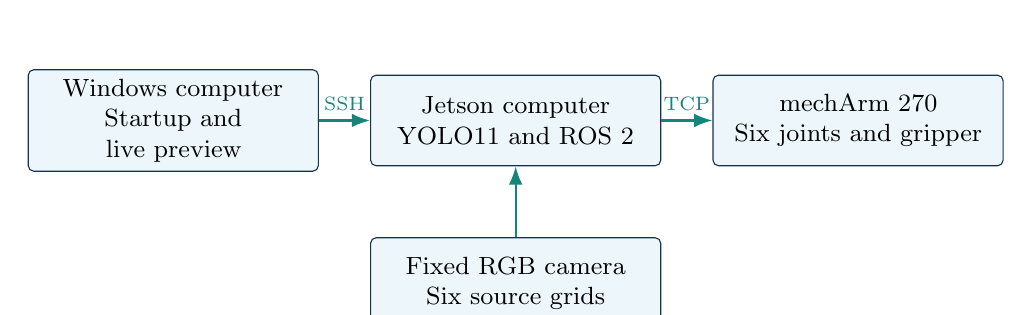
\begin{tikzpicture}[font=\small,>=Latex,
 box/.style={draw=Navy,rounded corners=2pt,align=center,minimum height=1.15cm,text width=3.45cm,fill=PaleBlue},
 arr/.style={->,thick,color=Teal}]
\node[box] (win) {Windows computer\\Startup and live preview};
\node[box,right=0.65cm of win] (jet) {Jetson computer\\YOLO11 and ROS 2};
\node[box,right=0.65cm of jet] (arm) {mechArm 270\\Six joints and gripper};
\node[box,below=0.9cm of jet] (cam) {Fixed RGB camera\\Six source grids};
\draw[arr] (win) -- node[above,font=\scriptsize]{SSH} (jet);
\draw[arr] (jet) -- node[above,font=\scriptsize]{TCP} (arm);
\draw[arr] (cam) -- (jet);
\end{tikzpicture}
\caption{Hardware and communication structure. The drawing summarizes the deployment shown in the defense presentation.}
\label{fig:hardware}
\end{figure}

The real scene contains colored objects, marked cells, the gripper, and background items such as cables and a power adapter. Cables and the adapter sometimes resemble targets and were included in the background training examples. The real photographs used in this report come from the Experiment 3 slides.

\begin{figure}[H]\centering
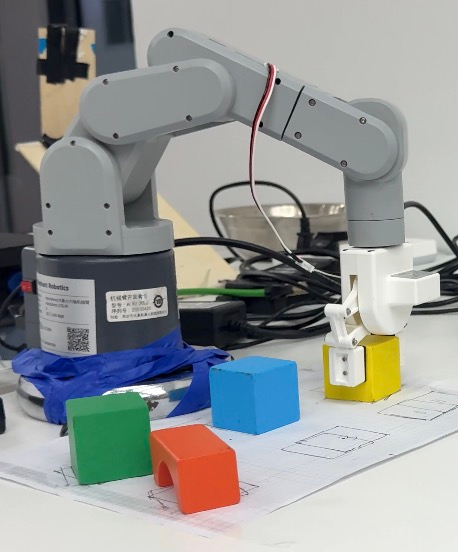
\includegraphics[height=6.0cm,keepaspectratio]{figures/robot_setup.png}
\caption{The mechArm and the tabletop objects in the supplied defense material, slide 7. The image shows the physical setup; it is not a measurement of position accuracy.}
\end{figure}

\subsection{Software modules and information flow}
The complete physical Launch file starts three ROS 2 nodes. The first node opens the camera, runs detection, publishes the raw image and detection array, and creates the preview and optional video. The second node maps detections to grids and runs the state machine. The third node receives one transfer request at a time and controls the arm.\src{integration,controller}

\begin{table}[H]\tabstart
\caption{Main software modules in the final physical pipeline}
\begin{tabularx}{\textwidth}{@{}L{5.75cm}Y@{}}
\toprule File or module & Main responsibility\\\midrule
\file{detector_node.py} & Camera input, YOLO boxes and labels, red/pink refinement, ROS publication, preview and video.\\
\file{experiment3_task_controller.py} & Grid assignment, stable group states, target selection, request tracking, timeout and task logs.\\
\file{experiment3_robot_worker.py} & Validate requests, run the transfer process, and return progress and completion feedback.\\
\file{experiment3_transfer_test.py} & Build the selected taught route, move the arm, check position and gripper feedback, and recover on errors.\\
\file{experiment3_region_}\newline\file{calibrator.py} & Create and check the six image polygons.\\
\file{experiment3_pose_recorder.py} & Record and save the named physical poses used by the six-grid task.\\
\bottomrule
\end{tabularx}
\end{table}

The image topic is \file{/camera/image_raw}, and the detection topic is \file{/yolo/detections}. A transfer request is sent on \file{/experiment3/transfer_requests}; worker responses return on \file{/experiment3/transfer_feedback}. The last two topics use JSON text inside ROS string messages. A request contains a request ID, grid ID, the detected six-class label after refinement, sorting group, destination, and detection confidence. The feedback links its status to the same request ID.

We use this request-and-feedback pair as the long-running task interface. It is implemented with topics rather than a ROS 2 Action server. The controller matches results by request ID and handles stale feedback and timeouts.

\subsection{Deployment, configuration, and module integration}
The supplied deployment process begins on Windows with configuration backup. The synchronization script downloads the active region polygons, gripper profiles, and 17-pose file from the original Jetson into the local package. This preserves the device settings before deployment. Changing the camera, robot base or gripper installation requires recalibration and pose checks.\src{integration,calibration,teaching}

The deployment script transfers the two ROS 2 packages, \file{yolo_detection_ros2} and \file{mecharm_pick_place}, into the Jetson workspace. It also uploads the hardware helpers, test scripts, model weights, and configuration files. On the Jetson, it sources ROS 2 Humble and runs \texttt{colcon build} with \file{--symlink-install} for these two packages. The startup script later sources both the ROS environment and the workspace installation, so ROS can find the built nodes.\src{integration}

The complete Launch file defines the active model, regions, poses, and gripper-profile paths in one place. The detector and controller receive the same region-file argument. This avoids displaying one set of grids while selecting actions from another. The active pose file and gripper profile belong to the same physical setup. 

The three node names are \file{experiment3_yolo_detector}, \file{experiment3_task_controller}, and \file{experiment3_robot_worker}. Their topic names provide fixed connections between modules. Windows opens an SSH tunnel from local port 18091 to Jetson preview port 8091, allowing the browser to show the remote image. The launcher checks for an existing robot controller and asks for one \texttt{RUN AUTO} entry before setting \file{armed:=true}. The Launch default is disarmed.\src{integration,controller}

Shutdown is also coordinated. Exit of the detector, controller, or worker triggers shutdown of the full Launch session. During cleanup, the worker attempts to stop an active runner, while the detector releases the camera and video resources. \src{integration,controller,vision}

A clear integration sequence is to check the connection and active files, build the packages, inspect the camera and grids in preview mode, and then check the taught routes and gripper settings through the dedicated tools. The complete run follows these module checks. Timestamped video and task logs then link visual decisions to requests and worker feedback.\src{integration,motion}

\subsection{Six labels and two destinations}
The detector retains six labels because the objects have different colors and shapes. The task controller reduces them to two movement groups. The distinction matters when a label is wrong. A blue-to-green cube error keeps the same destination. A pink-cube-to-red-cuboid error changes the destination.\src{vision,gripper}

\begin{table}[H]\tabstart
\caption{Class mapping and gripper targets}
\begin{tabularx}{\textwidth}{@{}L{4.7cm}C{1.6cm}C{2.3cm}Y@{}}
\toprule Detector label & Group & Destination & Closing target\\\midrule
\file{blue_cube} & cube & Right & 69\\
\file{green_cube} & cube & Right & 69\\
\file{pink_cube} & cube & Right & 69\\
\file{yellow_cube} & cube & Right & 69\\
\file{red_cuboid} & other & Left & 40\\
\file{orange_bridge} & other & Left & 40\\\bottomrule
\end{tabularx}
\end{table}

Both groups use an opening target of 100 and a gripper speed setting of 20. These values are device command values in the supplied profile. They are control values, not calibrated measurements of jaw angle or force. The profile is loaded from a configuration file so that a change in the gripper setup does not require rewriting the task logic.

\clearpage
\section{Simulation}
\label{sec:simulation}

\subsection{Robot model and scene}
The earlier Gazebo and MoveIt fixed-point pick-and-place project provided the development base. It established the robot model, collision scene, grasp approach, carrying motion, release, and return. Keyframe teaching and replay supported motion development before the six-grid task was integrated.\src{simulation}

The original \file{experiment3_sim_complete_20260914} used six red/blue cubes. The final extension, \file{experiment3_sim_bridge_20260921}, replaces the red cube in G2 and blue cube in G4 with two orange bridges. The six grid coordinates, other four objects, red/blue detection rules, original red/blue slots, and 65 mm carrying-centre height remain unchanged. The final scene has two red cubes, two blue cubes, and two bridges.\src{simcomplete,simbridge}

Each bridge is one 50 g rigid body with a crossbeam and two legs, three physical collision boxes, and a through-opening. Its envelope is $40\times40\times40$ mm; the opening is 20 mm wide and 28 mm high. Centre of mass and inertia are calculated from the component volumes. MoveIt conservatively uses the outer box for collision checking.

\begin{figure}[H]\centering
\begin{subfigure}{0.48\textwidth}
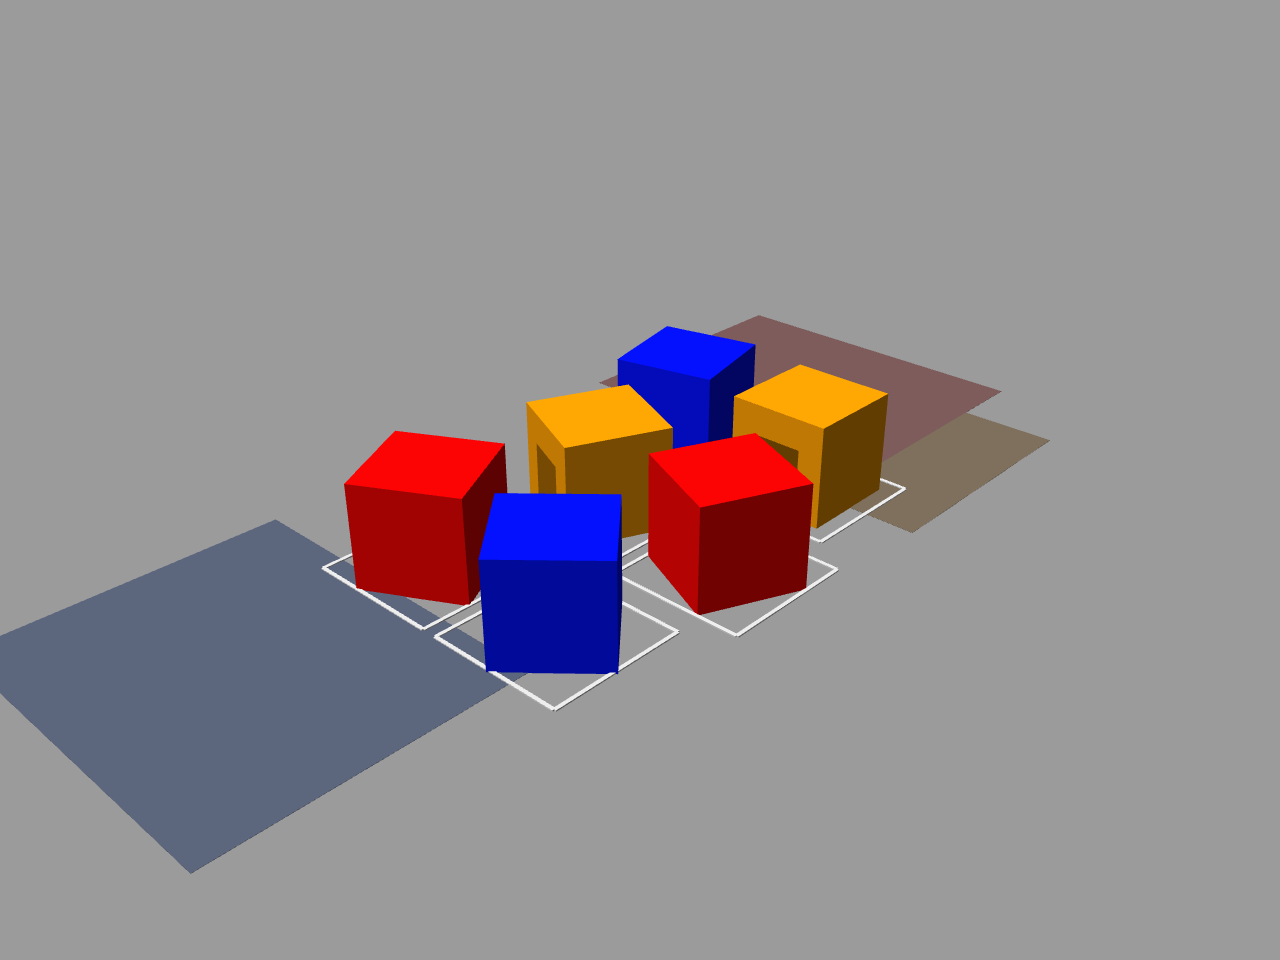
\includegraphics[width=\linewidth]{figures/simulation_bridge_initial.png}
\caption{Four cubes and two bridges in six source grids.}
\end{subfigure}\hfill
\begin{subfigure}{0.48\textwidth}
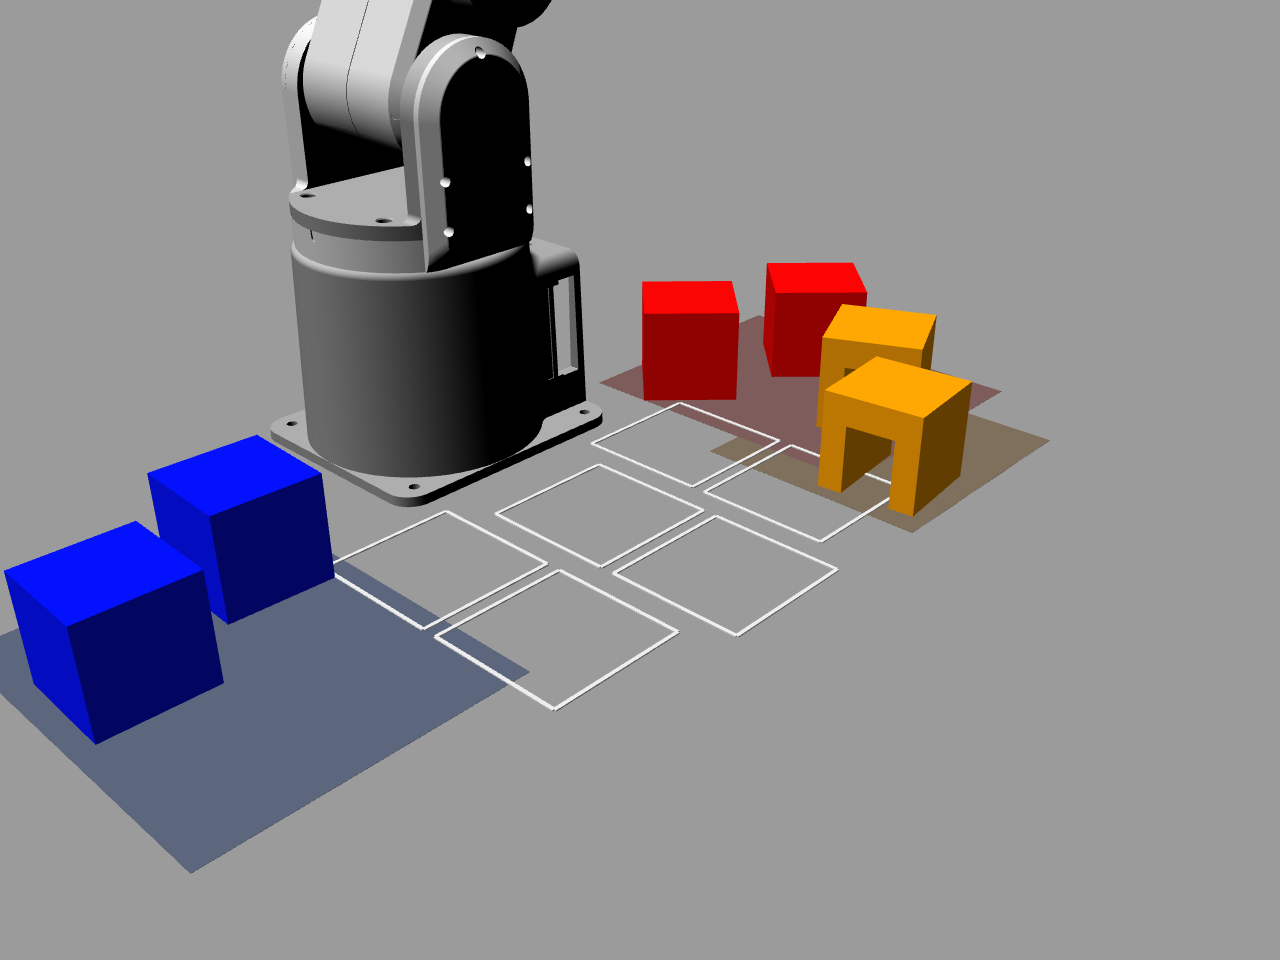
\includegraphics[width=\linewidth]{figures/simulation_bridge_final.png}
\caption{Final placement after six successful transfers.}
\end{subfigure}
\caption{Actual Gazebo side-camera images from the final bridge run. This observer camera does not participate in task decisions.}
\end{figure}

\subsection{Scene, image detection, and grid mapping}
The scene contains the mechArm, gripper, table, six fixed source cells, red/blue destination slots, added bridge slots on the left, and an overhead RGB sensor. The camera publishes a $960\times720$ image on \file{/task3/camera/overhead/image_raw}. The configured image rate is 8 Hz, not a measured processing rate.\src{simbridge}

The final simulation uses HSV segmentation and contour filtering for \file{red_cube}, \file{blue_cube}, and \file{orange_bridge}. It publishes class labels, boxes, and scores as \file{vision_msgs/Detection2DArray} on \file{/task3/detections}. Detection uses camera pixels, not scene ground-truth labels. Box centres are matched to projected grid regions and colors select destinations. This is color-associated classification, not color-independent shape recognition.\src{simbridge}

The simulation requires four consecutive matching grid observations and uses a configured minimum score of 0.65 before selecting a target. These settings belong to the HSV simulation pipeline. The physical system instead uses YOLO11 six-class detection, red/pink refinement, calibrated image polygons, and five-out-of-seven group voting. The two detectors and their scores are not interchangeable.

\subsection{Automatic control and motion feedback}
The simulation state machine contains \file{WAIT_READY}, \file{OBSERVE}, \file{SELECT}, \file{EXECUTING}, \file{VERIFY}, \file{RECOVER}, \file{DONE}, and \file{STOPPED}. The controller selects an eligible grid, submits one grasp job, waits for the result, allows the scene to settle, and then observes the remaining cells. The configured normal run processes each of the six grids once. It does not use the physical controller's refill policy.\src{simcomplete}

The grasp bridge exchanges request, status, result, and cancellation messages with job IDs. This is an equivalent feedback-based long-running task interface, rather than a standard ROS 2 Action server. Motion feedback and a 180 s controller job timeout prevent the controller from issuing another transfer while an earlier one is outstanding.

MoveIt plans the approach, grasp, lift, transfer, release, and return motions with collision objects. A simulation grasp check verifies alignment and gripper closure before attaching the object with a fixed constraint. This attachment supports carrying without snapping the object to a new pose; it is not a measurement of real friction or gripping force. Joint-state sampling and monitored physical contacts provide additional run checks.\src{simcomplete}

The complete system starts from one \file{full_sorting.launch.py}, including the scene, robot controllers, planning system, detector, grasp bridge, task controller, and independent acceptance monitor. The normal run does not require manual class, source-cell, or destination selection after startup.

\subsection{Final two-shape acceptance}
The final result is saved in \file{results/bridge_20260921_222016/acceptance.json}. Independent evaluation of actual Gazebo positions reports \file{PASS} and \file{DONE}: all six objects, including both bridges, are correctly placed. The evaluator checks the final position of each object.\src{simbridgerun}

\begin{table}[H]\tabstart
\caption{Object-level results of the final bridge simulation}
\begin{tabularx}{\textwidth}{@{}L{1.2cm}Y L{4cm}L{3cm}@{}}
\toprule Grid & Object & Target XY (m) & Independent result\\\midrule
G1 & Blue cube & $(0.170,0.070)$ & Correct\\
G2 & Orange bridge & $(-0.140,0.125)$ & Correct\\
G3 & Red cube & $(-0.170,0.070)$ & Correct\\
G4 & Orange bridge & $(-0.094,0.164)$ & Correct\\
G5 & Red cube & $(-0.112,0.045)$ & Correct\\
G6 & Blue cube & $(0.112,0.045)$ & Correct\\\bottomrule
\end{tabularx}\end{table}

The final run records 37,831 joint samples, zero joint-limit violations, zero monitored unsafe contact pairs, zero failed jobs, and a wall-clock duration of 391.53 s. The second bridge slot centre is just outside the source-grid edge, next to G4 after it has been emptied. Existing red/blue routing is preserved and remains different from the physical cube/other mapping.

Saved evidence includes configuration, world geometry, detections, job results, motion and safety logs, and two videos. The overhead video contains 1,354 frames encoded at 8 fps; the side video contains 651 frames at 5 fps. The videos use their configured encoding rates; the task duration comes from the run log.

\subsection{Historical normal and exception runs}
The normal record is \file{results/normal_front_arc_04/acceptance.json}. Independent evaluation of final object positions reports all six objects in their color-specific destinations: three red cubes and three blue cubes. The run finishes in \file{DONE}, with 37,412 joint samples, no recorded joint-limit violations, and zero contact pairs classified as unsafe by the monitor. Its recorded wall-clock duration is 466.26 s.\src{simruns}

\begin{table}[H]\tabstart
\caption{Recorded simulation results for the configured same-shape scene}
\begin{tabularx}{\textwidth}{@{}L{4.2cm}Y Y@{}}
\toprule Item & Normal run & Exception run\\\midrule
Run directory & \file{normal_front_arc_04} & \file{exceptions_front_arc_03}\\
Task state / evaluator status & \file{DONE} / \file{PASS} & \file{DONE} / \file{PASS}\\
Correct placements & 6 of 6 color-labeled cubes & 2 normal targets sorted; designated exception cells handled\\
Joint-state samples & 37,412 & 18,069\\
Recorded joint-limit violations & 0 & 0\\
Monitored unsafe contact pairs & 0 & 0\\
Wall-clock duration & 466.26 s & 238.73 s\\
\bottomrule
\end{tabularx}
\end{table}

The exception record is \file{results/exceptions_front_arc_03/acceptance.json}. Grid 2 contains an unknown-color object, grid 3 is empty, grid 5 has an injected unreachable-target condition, and grid 6 has an injected grasp failure. The controller skips the unknown and empty cells and handles the two motion failures through recovery. The remaining two ordinary targets are sorted. This run tests the designated exception branches; its two placements are not a normal-task sorting accuracy of two out of six.\src{simruns}

Both run directories preserve detections, task states, motion events, grasp-interface records, safety logs, initial/final images, and video. The independent evaluator checks actual final object positions rather than relying only on the controller's success count. 

\subsection{Debugging and remaining work}
The first bridge tests exposed an unreachable placement point and a Gazebo crash during release. We moved constraint operations to the physics-update thread and checked the distant slot with collision-free IK queries. Moving that slot inward allowed all six transfers to finish without lowering the carrying height.\src{simbridge}

After the accepted run, \file{move_group} logged a segmentation fault during SIGINT shutdown, while Gazebo exited normally. This shutdown issue remains to be resolved. The earlier exception tests cover the original scene; the bridge version has completed the normal run but has not repeated those exception tests.

\clearpage
\section{Visual Detection and Grid Mapping}
The detector, model metrics, and grid processing in this section apply to the physical experiment. The recorded simulation uses HSV color segmentation instead, as described in Section~\ref{sec:simulation}.

\label{sec:vision}

\subsection{Six-class detection and training method}

The vision system answers two questions before the robot moves: what kind of object is present, and which pickup cell contains it? We used YOLO11 to predict a class, a bounding box, and a confidence score for each object. The six labels were \file{blue_cube}, \file{green_cube}, \file{pink_cube}, \file{yellow_cube}, \file{red_cuboid}, and \file{orange_bridge}. The detector kept these labels for inspection, while the task controller reduced them to two sorting groups. The four cube classes went to the right area. The red cuboid and orange bridge went to the left area. In this project, ``v4'' means the fourth project model version, not the YOLOv4 network.\src{defense,vision}

The defense slides describe training with a $640\times640$ input, the AdamW optimizer, light data augmentation, and 35 epochs. Each training object had a class label and a box. The positive samples covered different colors, shapes, and views. We also included difficult background samples, such as an empty desk, cables, and the robot body. These negative samples helped the detector learn when it should produce no object box. This was useful because a background error could otherwise create a false pickup request.\src{defense}

The training, validation, and test sets had different roles. Training changed the model weights; validation helped select the saved weights; the test set checked detection quality after training. The selected model was then used for CUDA inference on the Jetson. Model evaluation results are given in Section 8.\src{defense}

Data quality was as important as the training settings. Boxes need to cover the object consistently, and labels need special care for red/pink views, touching objects, and partial occlusion. Background images should resemble the actual work area. Video frames close in time can be very similar, so a test on separately recorded scenes gives stronger evidence of general use than a random split of nearby frames. The supplied earlier data-building script uses time blocks for splitting; the final v4 dataset size is not stated here because a matching final dataset summary was not supplied.\src{vision}

\begin{figure}[H]
    \centering
    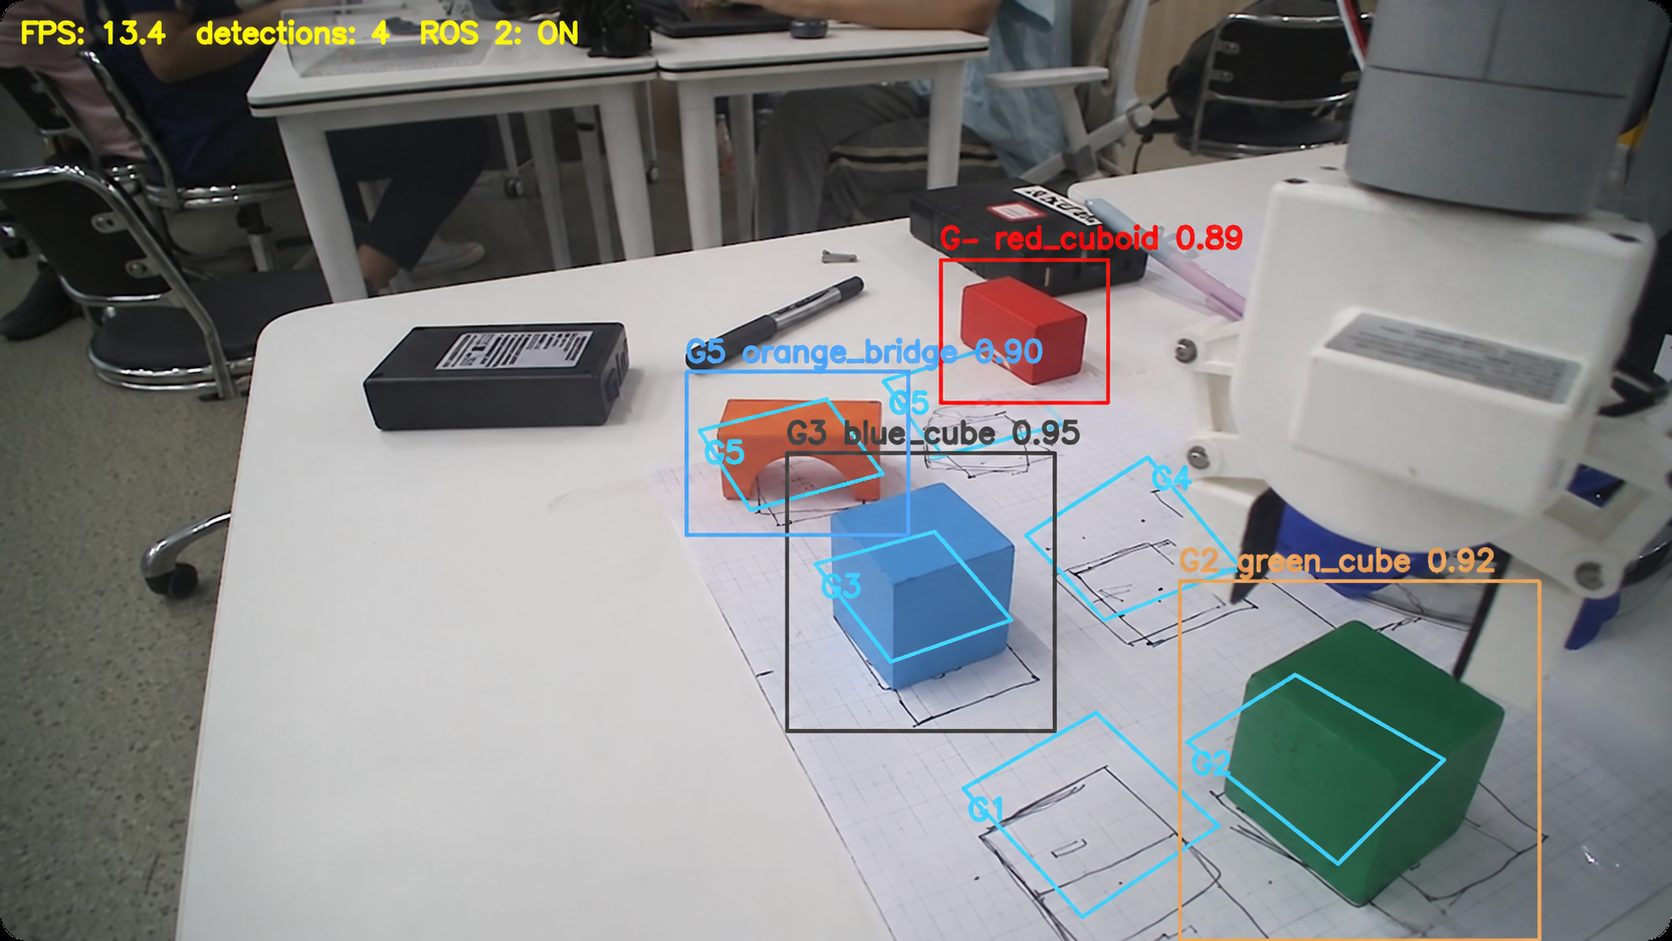
\includegraphics[width=0.92\textwidth]{figures/vision_scene.png}
    \caption{Detection and grid overlays in the experimental scene, reproduced from defense slide 4. Boxes show class names and confidence scores; blue polygons mark pickup regions. The displayed 13.4 FPS is one snapshot value, not a measured average over a complete run.\src{defense}}
    \label{fig:vision-scene}
\end{figure}

\Needspace{8\baselineskip}
\subsection{A second check for red and pink objects}

The red cuboid and pink cube were a difficult pair. Their colors could look similar under the camera, and a cuboid viewed from one end could appear nearly square. An error between these classes also changed the destination, so it deserved special attention. We therefore used the separate \file{red_pink_shape_classifier_v2.pt} model to check the object crop after the main detection.\src{vision}

For a pink or red detection, the program added padding equal to 8\% of the box width and height on each side. It kept the crop inside the image and passed it to the second model with an input size of 224. The correction rule was one way: an original pink-cube label changed to red cuboid only if the second model predicted red with a score of at least 0.55. An original red label was kept. The box position and main detector confidence were also kept.\src{vision}

The second classifier only processes candidate crops from the main detector, so it cannot recover an object that YOLO misses.

\subsection{Calibrating six image regions}

The table had six fixed pickup cells, named G1 to G6. Each cell was linked to taught robot poses. The camera therefore needed to select the correct cell, rather than calculate a new three-dimensional grasp pose for every object. The calibration program represented each cell by a four-corner polygon in the $1280\times720$ camera image. The operator clicked its corners in the browser view and then tested points inside and outside the regions.\src{calibration}

Before saving, the program checked that all six IDs were present, the corners were distinct and inside the image, and each polygon formed a valid convex quadrilateral. It rejected regions with an area below 1,000 square pixels and overlaps larger than two square pixels. These checks caught incomplete or poorly drawn regions before they reached the controller. The accepted polygons were stored in \file{regions.yaml}.\src{calibration}

The camera and table layout needed to stay fixed after this step. A change in camera position could move a visible cell even though its stored polygon stayed unchanged. Likewise, moving the robot base could break the link between a cell and its taught pose. The empty example configuration was only a template; the real experiment required the measured regions for its own setup.

\subsection{From a detection box to a pickup cell}

Let the top-left and bottom-right corners of a detected box be $(x_1,y_1)$ and $(x_2,y_2)$. Its image center is
\begin{equation}
    \mathbf{c}=(c_x,c_y)
    =\left(\frac{x_1+x_2}{2},\frac{y_1+y_2}{2}\right).
\end{equation}
For region polygon $P_i$, define the set of matching cells as
\begin{equation}
    \mathcal{G}(\mathbf{c})=\{i\in\{1,\ldots,6\}:\mathbf{c}\in P_i\}.
\end{equation}
The program assigns a grid ID only when $|\mathcal{G}(\mathbf{c})|=1$. A center outside all regions has no pickup cell. A center assigned to more than one region is also left unresolved. The controller uses a point-in-polygon calculation for this decision.\src{vision,controller}

Vision selects the cell, and the arm uses its stored approach and grasp poses. Objects need to stay near the taught pickup positions because this method does not estimate depth or adjust the grasp within a cell.

\begin{figure}[H]\centering
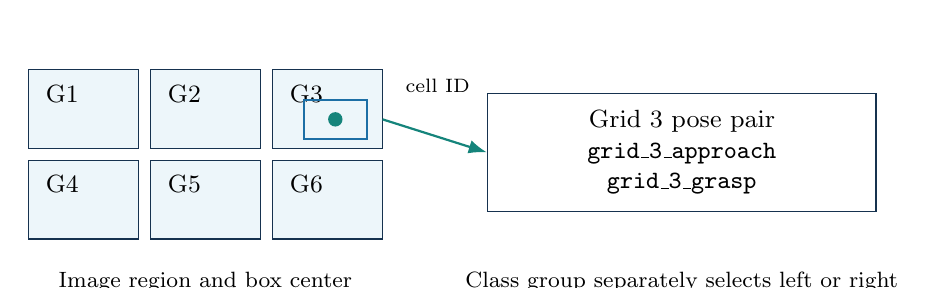
\begin{tikzpicture}[font=\small,>=Latex]
\foreach \id/\x/\y in {1/0/1.15,2/1.55/1.15,3/3.1/1.15,4/0/0,5/1.55/0,6/3.1/0}{
\draw[Navy,fill=PaleBlue] (\x,\y) rectangle ++(1.4,1.0);
\node[anchor=north west] at (\x+0.1,\y+0.93) {G\id};}
\draw[Blue,thick] (3.50,1.27) rectangle (4.30,1.77);
\fill[Teal] (3.90,1.52) circle (2.6pt);
\node[draw=Navy,align=center,text width=4.7cm,minimum height=1.5cm] (poses) at (8.3,1.1)
{Grid 3 pose pair\\\texttt{grid\_3\_approach}\\\texttt{grid\_3\_grasp}};
\draw[->,thick,Teal] (4.5,1.52)--(poses.west);
\node[font=\scriptsize] at (5.2,1.95) {cell ID};
\node[align=center,font=\footnotesize] at (2.25,-0.55) {Image region and box center};
\node[align=center,font=\footnotesize] at (8.3,-0.55) {Class group separately selects left or right};
\end{tikzpicture}
\caption{Discrete image-to-pose mapping. Grid 3 is an illustrative example; the drawing is a schematic, not the measured camera calibration.}
\end{figure}

\subsection{Stable decisions across several frames}

A box in one frame was not enough to trigger a pick. For each cell, the controller first converted the current detections into a sorting observation. No box gave \file{EMPTY}; an unsupported class gave \file{UNKNOWN}; and boxes from different sorting groups gave \file{MULTIPLE}. These unresolved cases did not become pickup targets.\src{controller}

The formal ROS controller treated several boxes from the same group as one group observation and used the highest-confidence box as its representative. This addressed cases where one physical cube produced overlapping boxes with different color labels. Since all cube labels shared a destination, those duplicate labels did not need different actions. The method still assumed one physical object per pickup cell: it could not distinguish duplicate boxes from two real objects of the same group.\src{controller}

The controller then stored the last seven observations, $o_{t-6},\ldots,o_t$. For each possible group or state $s$, it counted
\begin{equation}
    N_t(s)=\sum_{k=t-6}^{t}\mathbf{1}[o_k=s].
\end{equation}
After the window was full, a state was stable if it received at least five votes. Stable cube and other observations became \file{READY_CUBE} and \file{READY_OTHER}. Stable \file{EMPTY}, \file{UNKNOWN}, and \file{MULTIPLE} states were kept. If no state received five votes, the cell remained a candidate. Before issuing a request, the controller also required the current group to agree with the stable ready state. Voting was thus based on the sorting group, not an exact color label.\src{controller}

We set the detector confidence threshold to 0.25. Unique center-in-polygon assignment determines the source grid, and the controller requires five matching sorting-group observations in a seven-observation window. These checks suppress brief detection changes before a new target becomes ready.\src{vision,controller}

The confidence threshold, the NMS overlap threshold, and the temporal vote solve different problems. Confidence controls which candidate boxes are kept. NMS, configured with an IoU threshold of 0.45, reduces overlapping detections. The vote compares observations across frames. A lower confidence threshold can retain weak targets but also retain more false boxes. Persistent false detections can still pass these checks.

\section{Taught Poses and Robot Motion}
The taught poses, robot feedback, and gripper settings below belong to physical execution. Simulation uses the separate MoveIt and grasp-constraint workflow in Section~\ref{sec:simulation}.


\subsection{Recording the physical pickup and placement poses}

The fixed cells allowed us to use a small set of taught robot poses. After vision selected a cell and a sorting group, the worker loaded its pickup poses and the correct destination poses. This reduced the need to estimate a new three-dimensional grasp point from each image. It also made the limits clear: the camera, robot base, grid sheet, and gripper had to stay in their calibrated positions, and each object had to be placed near its cell center.\src{teaching,motion}

The physical recorder guided the operator through 17 named poses. It stored six joint angles and the tool center point (TCP) position and orientation for each pose. The source approach poses were taught above the objects; the grasp poses placed the fingers at the required pickup height. Both destinations had an approach pose and a lower release pose. A shared safe pose linked the source and destination routes.\src{teaching}

\begin{table}[H]\tabstart
\caption{The 17 named poses used by the physical task}
\begin{tabularx}{\textwidth}{@{}L{1.7cm}Y C{1cm}@{}}
\toprule Location & Pose names & Count\\\midrule
Shared & \file{safe} & 1\\
Grid 1 & \file{grid_1_approach}, \file{grid_1_grasp} & 2\\
Grid 2 & \file{grid_2_approach}, \file{grid_2_grasp} & 2\\
Grid 3 & \file{grid_3_approach}, \file{grid_3_grasp} & 2\\
Grid 4 & \file{grid_4_approach}, \file{grid_4_grasp} & 2\\
Grid 5 & \file{grid_5_approach}, \file{grid_5_grasp} & 2\\
Grid 6 & \file{grid_6_approach}, \file{grid_6_grasp} & 2\\
Left area & \file{left_approach}, \file{left_release} & 2\\
Right area & \file{right_approach}, \file{right_release} & 2\\\midrule
Total & One shared pose, twelve source poses, four destination poses & 17\\
\bottomrule
\end{tabularx}
\end{table}

The formal transfer code required a complete pose file and an active correction record covering all 17 points. It checked the angle limits and rejected invalid values before motion. The inherited simulation tools used RViz and the \file{q}/\file{qa}/\file{qb} keyframe method. They were useful for learning and checking motion ideas, while the physical Experiment 3 route used the named-pose recorder above. The two formats should not be treated as the same dataset.\src{teaching,motion,defense}

\subsection{Small joint steps and the transfer sequence}

The robot moved between taught joint targets using linear interpolation. Let $\mathbf q_0$ and $\mathbf q_1$ be two six-joint vectors, and let $\delta$ be the largest allowed command step. The program used
\begin{equation}
N=\max\!\left(1,\left\lceil\frac{\max_j|q_{1,j}-q_{0,j}|}{\delta}\right\rceil\right),
\qquad
\mathbf q_k=\mathbf q_0+\frac{k}{N}(\mathbf q_1-\mathbf q_0),\quad k=1,\ldots,N.
\end{equation}
Thus, no joint command changed by more than $\delta$ within one step. The final launch set $\delta=2^{\circ}$, a command interval of 0.20 s, and an SDK arm-speed value of 8. These are software settings; 8 is not a measured speed in degrees per second.\src{motion,integration}

The commands were sent in small steps, and feedback was checked at key poses. Joint interpolation did not guarantee a straight TCP path or impose a verified acceleration limit. We therefore relied on the taught layout, safe transition poses, and measured endpoint checks.\src{motion}

A transfer began at the safe pose with the gripper open. The arm moved above the selected cell, checked the open gripper, descended, and closed to the class-specific setting. After lifting, it checked the grip and returned through the safe pose. It then approached the selected destination, descended, released the object, lifted clear, and returned to safe. Figure~\ref{fig:motion-stages} shows three physical stages from the defense presentation.\src{motion,defense}

\begin{figure}[H]
\centering
\begin{subfigure}[t]{0.32\textwidth}
\centering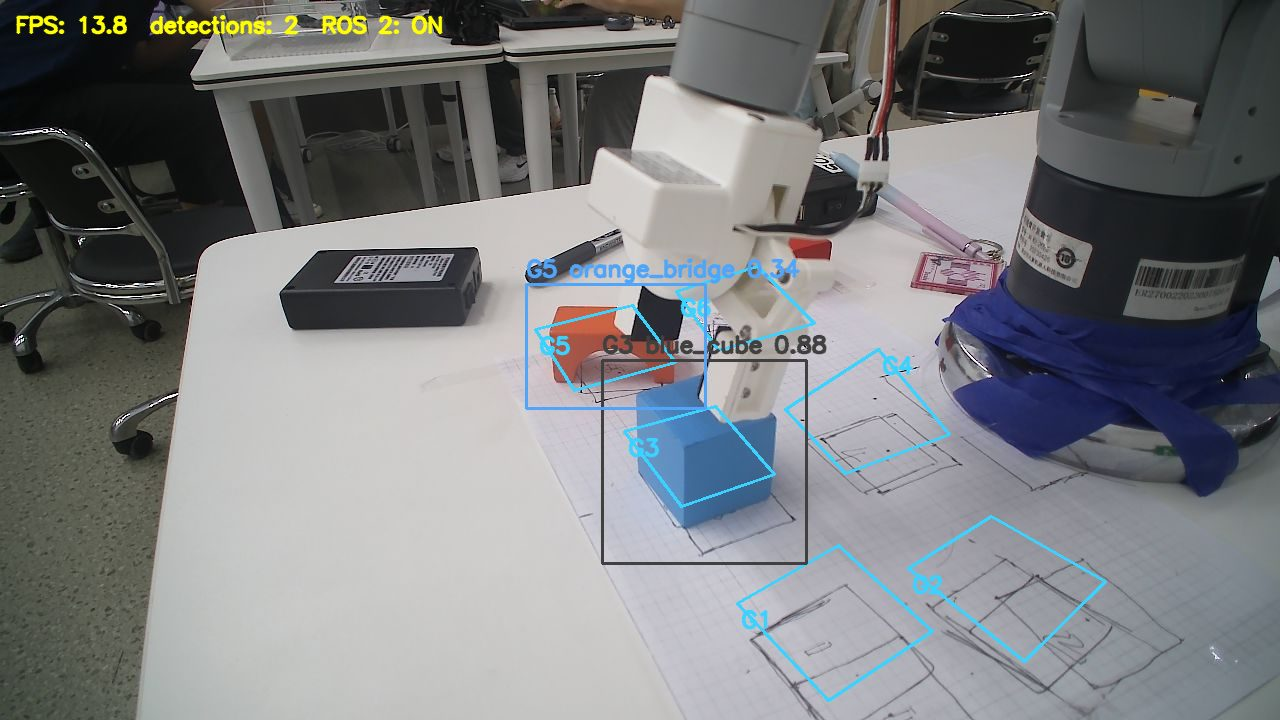
\includegraphics[width=\linewidth]{figures/approach.jpg}
\caption{Approach the source.}
\end{subfigure}\hfill
\begin{subfigure}[t]{0.32\textwidth}
\centering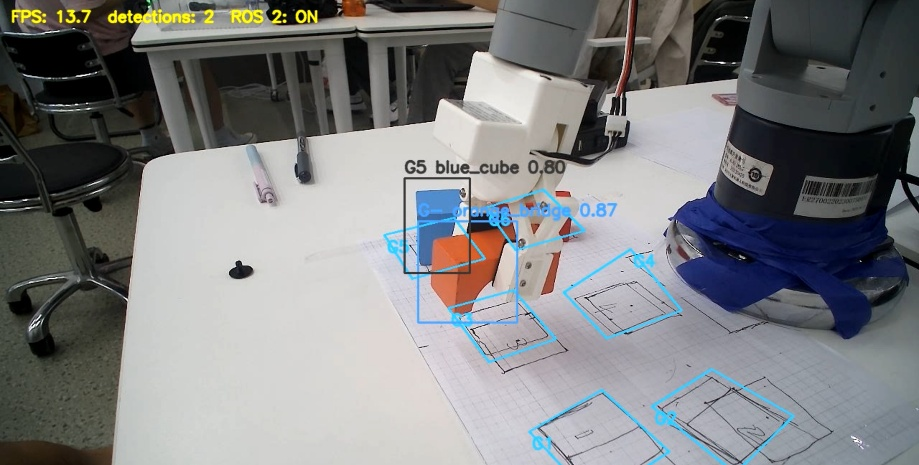
\includegraphics[width=\linewidth]{figures/grasp.jpg}
\caption{Descend and grasp.}
\end{subfigure}\hfill
\begin{subfigure}[t]{0.32\textwidth}
\centering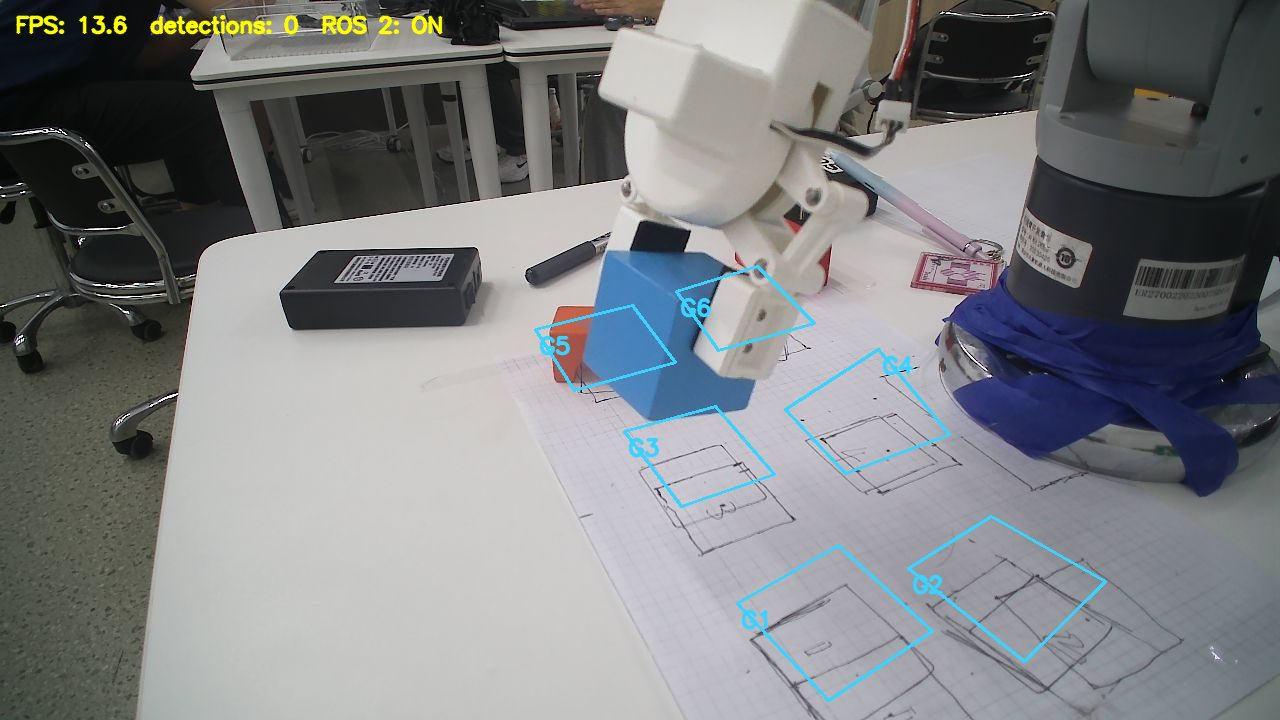
\includegraphics[width=\linewidth]{figures/lift.jpg}
\caption{Lift the object.}
\end{subfigure}
\caption{Physical motion stages shown in the supplied defense slides. These images illustrate the sequence; they do not provide a measured success rate.\src{defense}}
\label{fig:motion-stages}
\end{figure}

\subsection{TCP checks and clearance}

Sending a target did not mean that the arm had reached it. Before closing, the program waited for the TCP to settle near the grasp point. It sent the grasp route once, then read feedback without repeatedly sending the same joint target. Two consecutive acceptable samples were required. This reduced the chance of closing while the old arm was still moving.\src{motion}

\begin{table}[H]\tabstart
\caption{Selected motion acceptance settings, not measured positioning accuracy}
\begin{tabularx}{\textwidth}{@{}L{4.35cm}Y@{}}
\toprule Check & Configured condition\\\midrule
Ordinary grasp point & TCP horizontal error $\leq4$ mm; vertical error $\leq3$ mm.\\
Manually corrected grasp point & TCP horizontal error $\leq5$ mm; vertical error $\leq8$ mm.\\
Grasp stability & Two consecutive valid samples; up to nine checks at 0.75 s intervals.\\
Grasp joint guard & Other joint errors $\leq3^{\circ}$; joint 5 error $\leq8^{\circ}$.\\
Generated destination approach & Minimum clearance 50 mm; target 65 mm, also considering the highest recorded TCP position.\\
Post-release retreat & Measured TCP lift at least 75 mm, with a 0.5 mm feedback allowance.\\
\bottomrule
\end{tabularx}
\end{table}

The final code also adjusted difficult cells. It raised the requested grasp positions for grids 3 and 6 by 7 mm and 10 mm along their taught paths, and extended the grid 3 approach by 20 mm. These were generated targets, checked again through feedback. Since joint and Cartesian motion are not identical, the requested height change alone did not prove the physical result.\src{motion}

At the destination, the code could extend the taught release-to-approach direction to create a higher transition. After release, it checked the actual TCP height gain before returning across the workspace. These checks addressed low approach poses and the risk of touching the released object during departure. They still required a clear route and did not replace full obstacle detection.\src{motion}

\subsection{Class-specific gripping and delayed feedback}

One closing setting was not suitable for both object groups. The saved profile used OPEN=100, cube CLOSE=69, other CLOSE=40, and speed=20. These values use the gripper's control scale from 0 to 100; they are not angles or measured grip forces. The loader checked that the two close values were below the open value and that the profile was complete.\src{gripper}

The old gripper could respond late or stop briefly before reaching its final position. The program therefore checked visible feedback movement and several stable readings. For cube closing, the normal accepted feedback range was 64--72. A value of 73 was accepted only through a longer stable-contact check, requiring eight stable samples and enough closing movement. A brief pause at a more open position did not pass this check.\src{motion,gripper}

After lifting and before transfer, the program read the gripper position again without sending another close command. If an actuation failed, it could clear old commands and rebuild the control connection, with at most three sessions. Continued failure stopped the sequence. Position feedback was useful, but it could not measure grip force or prove that every object remained secure.\src{motion,gripper}

\subsection{Optional direction compensation}

An additional tool supported direction-based joint correction. For a joint approaching a pose from increasing or decreasing angles, it selected a matching correction and formed $q_{\mathrm{cmd},j}=q_{\mathrm{taught},j}+c_{j,d}$. This addressed the possibility that joint play and load caused different errors for different approach directions. When a joint target did not change, the previous direction was retained.\src{compensation}

The tool required validated settings, limited each correction to $3^{\circ}$, and supported a small preload movement. However, the supplied formal ROS worker did not enable this optional configuration by default. The main physical method was the corrected 17-pose route with feedback checks; the existence of the compensation tool does not establish a measured improvement in accuracy.\src{motion,compensation}

\section{Task Control and Exception Handling}
This section describes the physical controller, including its five-out-of-seven decisions and refill handling. The simulation controller uses four consecutive matching observations and a single pass over the six source grids; its state machine is described in Section~\ref{sec:simulation}.

\subsection{From a visual state to one transfer}
Each grid has a current visual state. A stable cube group becomes \file{READY_CUBE}; a stable non-cube group becomes \file{READY_OTHER}. Other states include \file{EMPTY}, \file{UNKNOWN}, \file{MULTIPLE}, and \file{CANDIDATE}. The controller chooses a ready target by ascending grid number. The current representative group must agree with the stable ready state. This prevents an old majority alone from creating a request when the current observation points to a different group.\src{controller}

\begin{figure}[H]\centering
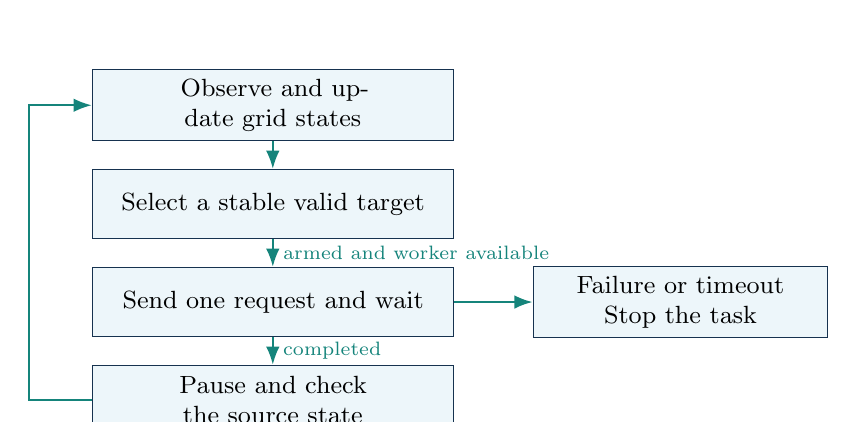
\begin{tikzpicture}[font=\small,>=Latex,
 b/.style={draw=Navy,fill=PaleBlue,align=center,text width=4.35cm,minimum height=0.88cm},
 a/.style={->,thick,color=Teal}]
\node[b] (observe) {Observe and update grid states};
\node[b,below=0.35cm of observe] (ready) {Select a stable valid target};
\node[b,below=0.35cm of ready] (run) {Send one request and wait};
\node[b,below=0.35cm of run] (verify) {Pause and check the source state};
\node[b,right=1.0cm of run,text width=3.5cm] (fail) {Failure or timeout\\Stop the task};
\draw[a] (observe)--(ready);
\draw[a] (ready)--node[right,font=\scriptsize]{armed and worker available}(run);
\draw[a] (run)--node[right,font=\scriptsize]{completed}(verify);
\draw[a] (run)--(fail);
\draw[a] (verify.west)--++(-0.8,0)|-(observe.west);
\end{tikzpicture}
\caption{Simplified task cycle. Non-target states are skipped; final completion also requires a stable empty scene.}
\end{figure}

The controller permits only one outstanding request. The worker also has a busy flag and checks that the grid lies in 1--6 and that the group matches the destination. It returns \file{STARTED}, \file{COMPLETED}, or \file{FAILED} with the request ID. Feedback for a different request is ignored by the controller. The worker sends \file{COMPLETED} only after the transfer routine returns without an error; that status describes software execution and its configured checks.

\subsection{Checking after a transfer}
After a completed transfer, the controller waits for the five-second interval and checks the source grid again. An \file{EMPTY} state accepts the transfer. A stable ready state also accepts the previous transfer and queues the current object again. This second rule supports immediate replenishment of a source cell.\src{controller}

A refilled cell and an unsuccessful pickup can produce the same ready state. We therefore checked placement in the video as well as the controller result.

The whole task ends automatically only after at least one transfer has been accepted, all six regions are stably empty, and that empty condition lasts for the configured five seconds. An initially empty table does not immediately finish the session. Unknown or mixed-group states also do not satisfy the all-empty completion condition, even though they do not trigger a pick.

\subsection{Exception states and recovery}
\begin{table}[H]\tabstart
\caption{Abnormal inputs and the implemented response}
\begin{tabularx}{\textwidth}{@{}L{3.1cm}Y@{}}
\toprule Condition & Controller or worker response\\\midrule
Empty cell & Record a skip and send no transfer request.\\
Unsupported class & Mark \file{UNKNOWN}, record a skip, and send no transfer request.\\
Conflicting groups in one cell & Mark \file{MULTIPLE}; do not select the cell.\\
Unstable observations & Keep \file{CANDIDATE} until a stable state is available.\\
Outside or ambiguous region & Assign no grid, so the detection cannot choose a route.\\
Disarmed mode or busy worker & Do not start a new movement; the worker rejects an invalid request.\\
Invalid pose, failed feedback check, or motion error & Raise a transfer error, attempt the programmed stop or recovery, and report failure.\\
Transfer exceeds 180 s & Record the timeout and stop the Launch through controller shutdown.\\
\bottomrule
\end{tabularx}
\end{table}

The complete Launch registers the exit of each main process. If the detector, controller, or worker exits, it requests shutdown of the remaining system. The worker attempts to stop an active runner during shutdown. A control lock also prevents two cooperating programs from commanding the same arm at once. Emergency-stop response time was not measured in these tests.\src{integration,motion}

\subsection{Unknown-object tests}
The project contains two related tests. The interface test publishes an unsupported label, \file{unrecognized_object}, at a selected cell center. It checks whether the controller enters \file{UNKNOWN}, records \file{SKIP_NO_MOTION}, and creates no transfer request. This isolates the task-control rule from detector quality.\src{unknown}

The physical unknown test first records an empty-cell background and then a scene with the test object. It uses a brightness-adjusted image difference to check occupancy. Its default criteria require a changed area of at least 3.5\% of the cell and a largest connected area of at least 2\%. It also requires no known-class detection in that cell. If these conditions hold, the test publishes the same unsupported label. Both test paths run the controller in disarmed mode and check for zero movement requests.

The occupancy test runs separately from normal six-class detection. During normal sorting, an unfamiliar object can still be missed or assigned a known label.

\section{Experimental Procedure and Configuration}
\subsection{Preparation and calibration}
The procedure connects the separately tested visual and movement parts. It begins with a fixed work area: the camera and robot base should not move after calibration, each source cell should contain at most one physical target, and the transfer and release areas should remain clear. A changed camera view changes the pixel polygons, while a changed robot or gripper setup changes the taught poses. These are separate reasons for recalibration.\src{calibration,teaching}

The deployment scripts distinguish the current device data from the software package. They provide a synchronization step for preserving the original Jetson's regions and poses before deployment. This matters because an empty example file is not a usable calibration. The supplied \file{regions.example.yaml} contains no actual region coordinates. A correct setup must recover the working \file{regions.yaml} and pose file from the device or collect them again.

For the visual module, the preparation sequence is:
\begin{enumerate}
\item Check that the six class names in the model and the controller have the same spelling and meaning.
\item Fix the camera at the required view and use the $1280\times720$ image for region calibration.
\item Mark four corners for each of the six source cells. Check the region IDs, polygon shape, area, and separation.
\item Put known objects in the cells and review the preview. Check both the class result and the grid result; one can be correct while the other is wrong.
\item Observe the empty scene and the backgrounds likely to appear during motion. Review false boxes on the table, cables, gripper, and nearby objects.
\item Check the group states across several frames before enabling robot execution.
\end{enumerate}

These steps describe the operating procedure supported by the tools. They do not add new test outcomes to the recorded defense results.

\subsection{Motion preparation and system startup}
The motion part needs the 17 named poses and the matching gripper profile. The route should first pass the available data checks and read-only precheck. Low-speed motion checks then establish whether the cell and destination poses match the physical arrangement. A successful visual preview alone does not validate reachability or clearance.\src{motion,teaching}

The complete physical launcher is \file{experiment3_real.launch.py}. Its default is \file{armed:=false}, which supports inspection before movement. The Windows \file{start_experiment3_ros2_auto.cmd} entry checks for an existing controller and asks for the initial \texttt{RUN AUTO} input. It then starts the complete ROS 2 Launch in armed mode. This initial enable step is distinct from manually selecting each object's class or route.\src{integration}

\Needspace{3\baselineskip}
During a normal cycle, the detector and controller choose the object, cell, and destination. The operator does not supply those decisions. The current launcher does, however, ask the operator to clear each released object during the five-second interval. The system supports automatic selection and transfer within this operating arrangement; it does not provide automatic stacking or management of a full destination area.

\subsection{Current physical Launch settings}
Table~\ref{tab:settings} records the supplied complete Launch configuration. The settings describe software inputs. They are not measured rates, motion accuracy, or a record of every value used during the earlier presentation run.\src{integration}

\begin{table}[H]\tabstart
\caption{Settings in the supplied complete physical Launch}\label{tab:settings}
\begin{tabularx}{\textwidth}{@{}L{4.55cm}L{2.4cm}Y@{}}
\toprule Setting & Value & Meaning\\\midrule
Camera image size & $1280\times720$ & Must match the region calibration.\\
Requested capture rate & 30 frames/s & Camera request, not measured inference speed.\\
Detector input size & 640 & Input scale used by the detector.\\
Detector confidence & 0.25 & Candidate detection threshold.\\
NMS IoU threshold & 0.45 & Box-overlap threshold used in duplicate suppression.\\
Red/pink correction threshold & 0.55 & Required specialist score for the implemented pink-to-red change.\\
History and stable votes & 7 and 5 & Group/state voting settings.\\
Inter-object interval & 5 s & Delay after a completed movement.\\
Empty-scene completion wait & 5 s & Required stable idle time after work has occurred.\\
Transfer timeout & 180 s & Maximum controller wait for one request.\\
Arm speed setting & 8 & Device motion setting used by the worker.\\
Maximum joint command step & $2^\circ$ & Bound used by joint interpolation.\\
Command period & 0.20 s & Delay between streamed targets.\\
\bottomrule
\end{tabularx}
\end{table}

\subsection{Records for analysis}
The system can save an annotated video, JSONL task events, and a motion log for each transfer. The most useful record joins the request ID with the grid, predicted class, selected group, destination, worker result, and visible placement outcome. This makes it possible to trace an incorrect placement back to recognition, mapping, or movement.\src{integration,controller}

For example, a correct label with a wrong grid suggests a spatial mapping problem. A correct grid with the wrong left/right choice suggests a class-to-group error. A correct request with an object still on the table suggests a physical execution problem. The present report uses this separation when interpreting results. New cycle times, per-object error values, and average frame rates are not estimated from isolated screenshots.

\section{Results and Analysis}
\subsection{Evaluation measures}
We evaluated image recognition, task execution and final placement separately. The detection metrics below describe model predictions; physical sorting results come from the videos and task records.

For detection, precision and recall can be written as
\begin{equation}
P=\frac{TP}{TP+FP},\qquad R=\frac{TP}{TP+FN},
\end{equation}
where $TP$ is a correct detection, $FP$ is a false detection, and $FN$ is a missed target under the evaluation matching rule. Precision helps describe false-target pressure; recall helps describe how many targets are found. Both are relevant to sorting. A false target may cause an unnecessary pick, while a missed object may remain on the table.

The overlap between a predicted box $B$ and a reference box $G$ is
\begin{equation}
\operatorname{IoU}(B,G)=\frac{|B\cap G|}{|B\cup G|}.
\end{equation}
mAP50 summarizes average precision with an IoU matching threshold of 0.50. mAP50--95 averages results over thresholds from 0.50 to 0.95 in steps of 0.05. The detector's mAP and the robot's transfer success rate measure different stages of the system.

\subsection{Simulation workflow results}
The final HSV simulation sorted four cubes and two bridges correctly: 6/6 total and 2/2 bridges. Independent acceptance recorded 37,831 joint samples, no joint-limit violations, no monitored unsafe contact pairs, and 391.53 s. Section~\ref{sec:simulation} provides all six object-level results and saved evidence.\src{simbridgerun}

The two geometries completed the same pickup and placement sequence. The HSV detector and fixed-constraint grasp model are described in the simulation chapter.

\subsection{Offline model results}
The model results available from training and the defense presentation are listed below. The v3 baseline includes four metrics; the v4 result gives mAP50--95.\src{defense}

\begin{table}[H]\tabstart
\caption{Detector results reported in the defense presentation}
\begin{tabularx}{\textwidth}{@{}L{3.8cm}*{4}{>{\centering\arraybackslash}X}@{}}
\toprule Model and source & Precision & Recall & mAP50 & mAP50--95\\\midrule
v3 baseline, slide 9 & 0.9505 & 0.9342 & 0.9360 & 0.8699\\
Final v4, slide 4 & Not stated & Not stated & Not stated & 0.8755\\
\bottomrule
\end{tabularx}
\end{table}

The recorded mAP50--95 increased from 0.8699 to 0.8755, a difference of 0.56 percentage points. The v4 training added field images and difficult backgrounds. The available summary results do not isolate the contribution of individual training changes.

The red/pink classifier achieved 94.12\% Top-1 accuracy on 68 test crops: 26 pink and 42 red. In the running pipeline, it changes a pink prediction to red only when its score reaches the configured threshold. The crop test does not include missed detections or grid-assignment errors.\src{classifiermetrics}

\subsection{Physical sorting demonstration}
With the instructor's approval, we started the physical test with five objects and re-fed the yellow cube once, producing six transfers. The acceptance video shows the red cuboid, yellow cube, re-fed yellow cube, blue cube, orange bridge, and green cube delivered to their corresponding sorting areas. Four cube transfers go right and two non-cube transfers go left. All six transfers went to the intended sorting area; the group recorded no failed transfer.\src{physicalvideo}
\begin{equation}
S_{\mathrm{cycles}}=\frac{6\text{ matching destination choices}}{6\text{ transfer cycles}}=100\%.
\end{equation}

\begin{table}[H]\tabstart
\caption{Observed acceptance-video cycles}\label{tab:physicalobjects}
\begin{tabularx}{\textwidth}{@{}L{1.2cm}Y L{1.5cm}L{2.9cm}L{3cm}@{}}
\toprule Cycle & Visible object & Area & Grasp/transport & Delivery interval\\\midrule
P01 & Red cuboid & Left & Observed & 00:22--00:25\\
P02 & Yellow cube & Right & Observed & 01:16--01:19\\
P03 & Re-fed yellow cube & Right & Observed & 02:04--02:06\\
P04 & Blue cube & Right & Observed & 02:48--02:49\\
P05 & Orange bridge & Left & Observed & 03:22--03:24\\
P06 & Green cube & Right & Observed & 03:59--04:01\\
\bottomrule
\end{tabularx}
\end{table}
The intervals refer to \file{2eb7001d38fd861630d52918161ba8cf.mp4} and use approximate playback timestamps. The operator re-feeds the yellow cube and clears delivered objects. Cycle IDs describe transfer order rather than six distinct physical objects.

\begin{figure}[H]
\centering
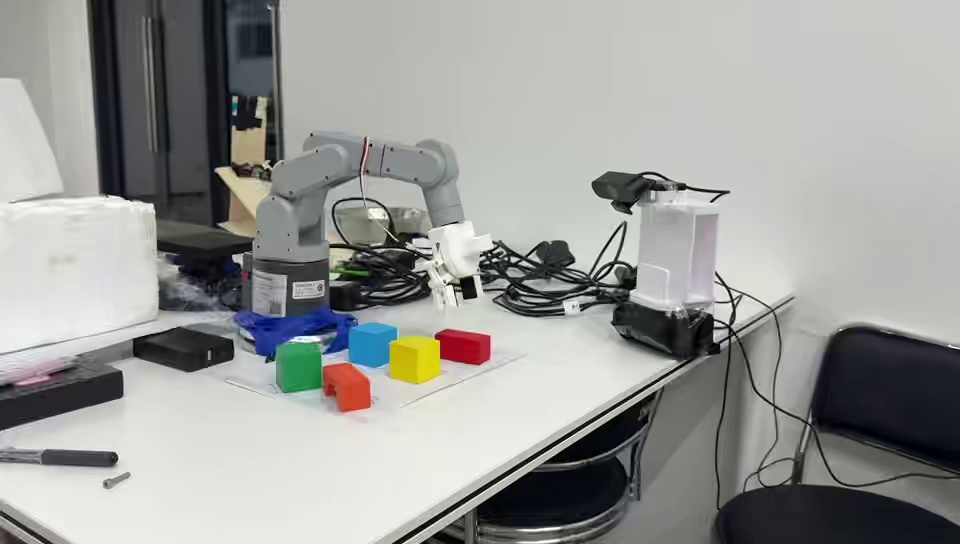
\includegraphics[width=0.47\textwidth]{figures/physical_acceptance_initial.jpg}\hfill
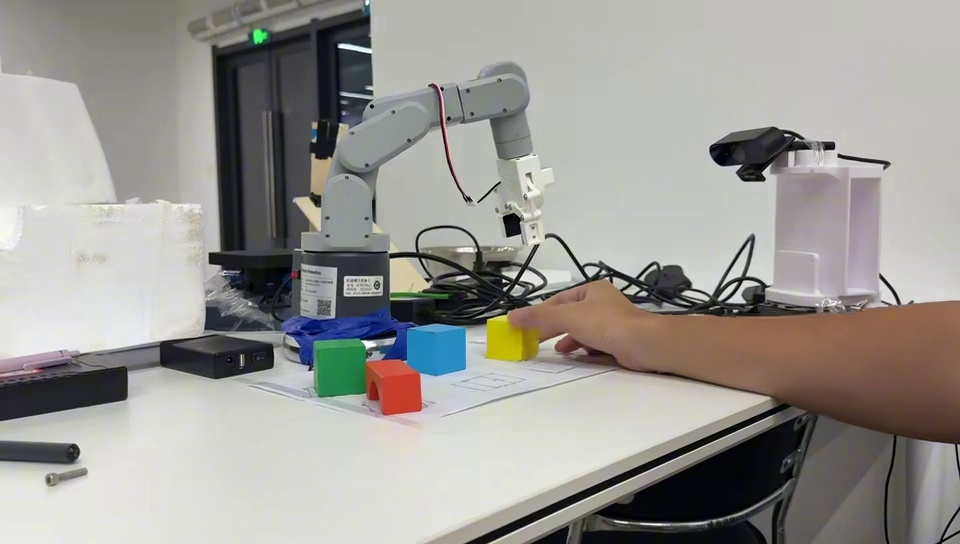
\includegraphics[width=0.47\textwidth]{figures/physical_acceptance_refeed.jpg}
\caption{Physical acceptance: initial scene and yellow-cube re-feed at approximately 01:24.}
\end{figure}

\subsection{Original task records}
The task JSONL for 2026-09-08 03:25:15 records an armed controller, six transfer requests, six completed worker results, six accepted transfers, and final \file{completed_count=6}. Its chronological source grids are G1, G3, G2, G4, G5, and G6. Request IDs connect source selection, destination, worker feedback, and source-clear verification.\src{physicalrecords}

\begin{table}[H]\tabstart
\caption{Six-cycle task log}
\begin{tabularx}{\textwidth}{@{}L{1.4cm}L{1.4cm}Y L{2cm}L{2.6cm}@{}}
\toprule Request & Grid & Recorded detector label & Area & Worker result\\\midrule
1 & G1 & \file{orange_bridge} & Left & COMPLETED\\
2 & G3 & \file{yellow_cube} & Right & COMPLETED\\
3 & G2 & \file{yellow_cube} & Right & COMPLETED\\
4 & G4 & \file{blue_cube} & Right & COMPLETED\\
5 & G5 & \file{orange_bridge} & Left & COMPLETED\\
6 & G6 & \file{green_cube} & Right & COMPLETED\\
\bottomrule
\end{tabularx}
\end{table}
The table lists detector outputs. The video table above instead describes visible object shapes and playback times; the source files are identified with each record.

The v4 task of 2026-09-07 19:26:01 is a separate five-transfer run, covering G1, G2, G3, G5, and G6. G4 remained without a stable target. Its final count is five. The matching visual-recognition AVI shows the detector overlays and five-object scene; these records are not added to the six-cycle total.

\subsection{Empty and unknown targets}
Recovered physical-unknown tests at 15:38:52 and 19:50:38 on September 7 record G1 as \file{UNKNOWN} and then \file{SKIP_NO_MOTION}, with no transfer request. Empty cells are also skipped. Both tests use a disarmed controller to inspect the visual and task-decision branches. An additional interface-injection test records the unsupported-class path. Original JSONL, console outputs, and evidence images are included.\src{physicalrecords}

\subsection{Red-cuboid and orange-bridge refinement}
The detector includes a \file{red_orange_pair_classifier_v2.pt} stage for candidates labelled \file{red_cuboid} or \file{orange_bridge}. A result is accepted when its confidence is at least 0.80 and its lead over the second class is at least 0.30. Otherwise, the main detector label is retained. This refinement changes the fine class while preserving the shared left-side sorting group.\src{pairrefinement}

The classifier test produced 84/84 correct crops. In a video regression of 36 detections, 20 red-cuboid cases change from bridge labels to red-cuboid labels, and 16 bridge cases remain correct. Both evaluations used saved image data; the updated classifier has not been evaluated in a new physical acceptance run.

\subsection{Operating settings}
The main detector confidence is 0.25; NMS IoU is 0.45. Detection-box centers determine unique polygon ownership. A seven-observation history requires at least five matching sorting-group votes, with the current group also matching before a target is ready. The controller routes \file{cube} right and \file{other} left.\src{controller,integration}

The classification gripper profile is \file{OPEN=100}, \file{cube CLOSE=69}, \file{other CLOSE=40}, and speed 20. The calibration files provide 17 measured reference poses and directional correction data. Before operation, the region layout and poses are checked against the current setup.\src{motion,gripper}


\Needspace{0.58\textheight}
\section{Main Problems and Solutions}
\label{sec:problems}
\lead{Recognition and grid stability.} A red/pink classifier reduced confusion between similar objects. Calibrated grid polygons and five-out-of-seven group voting stabilized cell selection.\src{vision,calibration,controller}

\lead{Position and gripper errors.} We corrected taught poses and checked TCP and gripper feedback during transfer. Continued failure triggered recovery or shutdown.\src{teaching,motion,gripper}

\lead{Task coordination.} A control lock, request IDs and worker feedback kept transfers in order, with only one motion request active at a time.\src{controller,integration}

\lead{Empty and unknown cells.} Empty cells were skipped. A separate unknown-object test used occupancy comparison and an unsupported-class message to check that no movement request was issued.\src{unknown,controller}

\lead{Simulation extension.} An unreachable bridge destination was repositioned, and constraint operations were moved to the Gazebo update thread to fix a release-stage crash. The task then passed 6/6. A MoveIt shutdown error after acceptance remains unresolved.\src{simbridge,simbridgerun}

\section{Conclusion}
The system completed the required sequence from camera detection to grid selection, grasping and classified placement. Fixed pickup grids allowed us to use taught poses while leaving object selection and destination choice to the controller.

In simulation, four cubes and two bridges reached their assigned positions. On the physical arm, the instructor-approved test used five initial objects and one re-feed to complete six transfers. Original task logs record the six requests and completed results. Empty and unknown cells were checked in separate no-motion tests.\src{simbridgerun,physicalvideo,physicalrecords}

The main implementation choices were five-of-seven group voting, one motion request at a time, and position and gripper checks during transfer. Red/pink and red/orange classifiers were added for the object pairs that caused recognition errors. The red/orange update has been evaluated on saved images and video. Further physical trials would be needed to measure its effect on repeated sorting runs.

\clearpage\appendix
\section{Physical Sorting Cycle}
The physical sorting loop is outlined below. Motion routines handle retries and feedback checks.

\begin{lstlisting}[caption={Main stages of the complete physical task}]
Load the active models, regions, taught poses, and gripper profiles
Validate the configuration and start detector, controller, and worker
Acquire the robot control lock before armed operation
While the task is active:
    Update the stable states of all six source cells
    Log non-target states without requesting a movement
    If a transfer is running:
        Wait for feedback with the matching request ID
        On failure or timeout: stop the task and record the cause
    Else if a completed transfer needs source verification:
        Wait for the inter-object interval
        Accept EMPTY, or accept and requeue a stable ready cell
        Continue waiting for an unresolved source state
    Else if an eligible cell exists and the task is armed:
        Choose its group and destination automatically
        Send one transfer request to the worker
        Validate the selected route and open the gripper
        Move safe -> source approach -> source grasp
        Check the grasp pose, close, lift, and check the hold
        Move through safe to the selected destination
        Descend, release, verify clearance, and return to safe
        Report COMPLETED or FAILED with the motion-log path
    Else if work occurred and all cells stayed empty for 5 seconds:
        Complete the session
On exit: stop any active runner and close cameras and connections
\end{lstlisting}

A ready cell after transfer can mean either refill or an object left behind. The outline therefore preserves the current requeue rule without treating it as independent proof of physical success. The final placement must be checked using the video or another outcome measurement.

\clearpage
\section{Visual Processing Logic}
The detector and controller logic is shown below. The robot worker executes the selected request. Here, UNKNOWN means an unsupported received label.

\begin{lstlisting}[caption={Visual processing and request selection in the supplied ROS pipeline}]
Load detector v4, red/pink v2, red/orange pair v2, and six polygons
Create a history of length 7 for each cell
For each camera frame:
    boxes = detect(frame, size=640, confidence=0.25, nms_iou=0.45)
    For each pink or red box:
        crop = crop_with_padding(frame, box, padding=0.08)
        label, score = classify(crop, size=224)
        If box is pink and label is red and score >= 0.55:
            change the class to red
    For each remaining red-cuboid or orange-bridge candidate:
        Run the red/orange pair classifier
        If confidence >= 0.80 and top-two margin >= 0.30:
            adopt the pair classifier label
    Publish classes, scores, box centers, and sizes
    Assign boxes to cells by unique center-in-polygon match
    For each cell:
        If no box: observation = EMPTY
        Else if an unsupported class exists: observation = UNKNOWN
        Else if known groups differ: observation = MULTIPLE
        Else: observation = shared group; choose highest-score box
        Update the seven-observation history
        If seven entries exist and at least five agree:
            stable = the majority group or state
        Else: stable = CANDIDATE
        A group is ready only if the current group also agrees
    If armed, idle, and the required waits are complete:
        Select the lowest-numbered ready cell
        Send one request: cube -> right; other -> left
\end{lstlisting}

\clearpage
\section{Submission File Index}
\label{sec:submission}
The submission folder is \file{Group15_Experiment3_Compact_20260924}. The root \file{README_CN.md} describes the package contents and \file{SHA256SUMS.txt} records file checksums. Video encoding and original-file identities are listed in \file{VIDEO_COMPRESSION.md}.

\begin{longtable}{@{}L{3.1cm}L{5.8cm}L{6.1cm}@{}}
\caption{Submission directory guide}\\
\toprule Material & Relative path & Contents\\\midrule\endfirsthead
\toprule Material & Relative path & Contents\\\midrule\endhead
\bottomrule\endfoot
Group report & \file{01_Report/} & PDF, LaTeX source, and figures\\
Physical implementation & \file{02_Physical/} & ROS 2 detector, task controller, robot worker, hardware tools, Launch and deployment scripts\\
Models & \file{02_Physical/models/} & Main v4 detector, red/pink v2 classifier, red/orange pair v2 classifier\\
Classification settings & \file{02_Physical/config/class_mapping.yaml}, \file{gripper_profiles.yaml} & Class routing and gripper targets\\
Latest simulation & \file{03_Simulation/experiment3_sim_bridge_20260921/} & Six grids, four cubes and two bridges; code, videos and independent acceptance\\
Historical simulation & \file{03_Simulation/experiment3_sim_complete_20260914/} & Original normal and exception runs\\
Reviewed physical videos & \file{04_Evidence/Physical_Video/} & Acceptance MP4 and separate visual-recognition MP4 (compressed from AVI)\\
Original physical records & \file{04_Evidence/RawRuns/} & Six-cycle task, five-cycle v4 task, physical UNKNOWN and injection tests, console logs, images and videos\\
Task and video indices & \file{05_Records/} & Original request association index and video-cycle observations\\
Measured pose reference & \file{06_Calibration/measured_17poses_20260907.yaml} & Seventeen recorded robot poses for calibration reference\\
Direction compensation & \file{06_Calibration/joint_compensation.yaml} & Recorded directional correction data\\
Training and evaluation & \file{07_Training/} & Main detector training material and red/orange refinement datasets, scripts and evaluations\\
\end{longtable}

\subsection{Reading the results}
The final bridge simulation record is \file{03_Simulation/experiment3_sim_bridge_20260921/results/bridge_20260921_222016/acceptance.json}: six correct placements, including both bridges, with 37,831 joint samples. Its two videos and original event records are stored in the same run directory.

Physical request records preserve the original grid IDs, detector labels, destinations and worker feedback. The six-cycle and five-cycle runs retain separate identities. Video observations describe visible object transfers; offline classifier evaluations describe image-classification performance. 

\subsection{Configuration and use}
The classification workflow uses main-detector confidence 0.25, seven-observation/five-vote sorting-group stability, unique center-in-polygon grid assignment, and cube/right versus other/left routing. Gripper values are OPEN 100, cube CLOSE 69, other CLOSE 40, and speed 20. Configuration examples and calibration tools accompany the source.

The measured-pose reference is retained in the calibration directory without replacing the robot's runtime configuration. Before physical operation, perform the documented region calibration, pose checks and low-speed validation for the current setup. 

\clearpage
\addcontentsline{toc}{section}{References}
\begin{thebibliography}{99}
\small\raggedright
\setlength{\baselineskip}{10.4pt}
\setlength{\itemsep}{1pt}
\setlength{\parskip}{0pt}
\bibitem{requirements}
Robot Integration Group Project I. \emph{Experiment 3 Desktop Object Classification and Sorting: Simulation and Physical Verification Requirements}. Laboratory handout and report-format requirements, in Chinese.

\bibitem{defense}
Group 15. \emph{Experiment 3 Desktop Object Classification and Sorting}. Defense presentation, 10 slides. Visual module: slides 4--5; motion and results: slides 6--9. The chart on slide 9 records the v3 baseline.

\bibitem{lab2}
Zhang Feixiang. \emph{Experiment 2 Fixed-Point Robotic Pick-and-Place}. Individual experiment report, 2026.

\bibitem{vision}
Project visual implementation. \file{detector_node.py}, \file{experiment3_vision_preview.py}, and \file{class_mapping.yaml}. Training context: the local \file{cube_detection} project, including its README and \file{scripts/build_dataset.py}.

\bibitem{calibration}
Project grid calibration. \file{experiment3_region_calibrator.py}, \file{regions.example.yaml}, and the region-configuration README.

\bibitem{controller}
Project task control. \file{experiment3_task_controller.py} and \file{experiment3_robot_worker.py}. ROS 2 implementation.

\bibitem{teaching}
Project teaching tools. \file{experiment3_pose_recorder.py}, \file{mecharm_real_recorder.py}, and \file{MANUAL_TEACHING_CN.md}.

\bibitem{motion}
Project physical motion. \file{experiment3_transfer_test.py}, \file{experiment3_grid_dry_run.py}, \file{experiment3_grid_grasp_test.py}, \file{experiment3_all_grid_sequence.py}, and \file{mecharm_recorded_task.py}.

\bibitem{gripper}
Project gripper configuration. \file{gripper_profiles.yaml}, \file{experiment3_gripper_profiles.py}, and \file{experiment3_gripper_profile_tester.py}.

\bibitem{compensation}
Project optional joint correction. \file{experiment3_directional_compensation.py}.

\bibitem{integration}
Project deployment and startup. \file{experiment3_real.launch.py}, the complete-system README, Windows deployment and synchronization scripts, and \file{start_experiment3_ros2_auto.cmd}.

\bibitem{unknown}
Project exception tests. \file{experiment3_unknown_exception_test.py}, \file{experiment3_physical_unknown_test.py}, and their corresponding \file{run_experiment3_*_test.sh} launch scripts.

\bibitem{simulation}
Project simulation and keyframe base. \file{experiment.launch.py}, \file{teaching.launch.py}, \file{task_executor.py}, \file{keyframe_player.py}, \file{task_points.yaml}, Gazebo world/model files, and the simulation README.

\bibitem{classifiermetrics}
Project saved classifier evaluation. \file{cube_detection/models/red_pink_classifier_v2_metrics.json}. Two-class test split with 26 pink and 42 red crops; reported Top-1 accuracy 94.12\%.
\bibitem{simcomplete}
Group 15. Baseline simulation source, \file{experiment3_sim_complete_20260914}: Launch, configuration, detector, controller, grasp bridge, motion and acceptance monitor.

\bibitem{simruns}
Group 15. Baseline records in \file{experiment3_sim_complete_20260914/results/normal_front_arc_04/} and \file{exceptions_front_arc_03/}: acceptance, logs and videos for normal sorting and designated exceptions.

\bibitem{physicalarchive}
Group 15. Combined Experiment 2/3 core-code archive, dated 2026-09-13. Physical code in \file{02_Physical/}, including ROS packages, detector models, class mapping, gripper profiles and deployment tools.

\bibitem{simbridge}
Group 15. Six-grid bridge extension, \file{experiment3_sim_bridge_20260921}: configuration, world generator, grasp plugin, detector, motion and retained development runs.

\bibitem{simbridgerun}
Group 15. Final bridge run, \file{experiment3_sim_bridge_20260921/results/bridge_20260921_222016/}: independent acceptance, configuration, geometry, per-job evidence and two camera videos.

\bibitem{physicalvideo}
Group 15. Physical video records in \file{04_Evidence/Physical_Video/}: visual-recognition demonstration \file{acceptance_20260907_192601.mp4} (compressed from the original AVI), and acceptance video \file{2eb7001d38fd861630d52918161ba8cf.mp4}. Original identities and encoding details: \file{VIDEO_COMPRESSION.md}.

\bibitem{physicalrecords}
Group 15. Physical task JSONL, console logs, and UNKNOWN-test images. Six-cycle task: 20260908\_032515; five-cycle v4 task: 20260907\_192601. Included in \file{04_Evidence/RawRuns/}; request association in \file{05_Records/task_index.json}.

\bibitem{pairrefinement}
Group 15. Red-cuboid/orange-bridge pair classifier v2, detector integration, and saved offline evaluation reports. Code and weights in \file{02_Physical/}; training and regression evidence in \file{07_Training/}. Crop test: 84/84; video regression: 36/36 evaluated detections.

\end{thebibliography}

\end{document}
